\section{Clustering}
	Al fine di trovare eventuali differenze o similitudini significative tra i record del dataset, dopo le operazioni di comprensione e preparazione dei dati, sono stati applicati su di essi tre algoritmi di clustering differenti, ovvero K-means, DBSCAN e Agglomerative Hierarchical.$\newline$
	In questo capitolo si descrivono i metodi usati e i risultati ottenuti.

\subsection{Clustering con K-means}
	Il primo algoritmo applicato sui dati è il k-means. Esso permette di ottenere un center-based clustering, in cui cioè, ogni cluster è individuato da un punto centrale detto centroide e ogni altro punto è assegnato al cluster con il più vicino centroide. Tale algoritmo richiede che sia fissato in precedenza il numero k di clusters che si vogliono ottenere.$\newline$
	%\subsubsection{Scelta degli attributi e della funzione di distanza}
	Per la misura della distanza tra i punti si è scelto di usare la distanza euclidea poiché è su di essa che si basa il Lloyd's algorithm, ovvero l’algoritmo standard originario da cui deriva il k-means a cui ancora oggi ci si può riferire con entrambi i termini. Per poter applicare l’algoritmo k-means è stato creato un dataset di training che contiene tutti i record e gli attributi del dataset originario, fatta eccezione per gli attributi categorici e binari e per l’attributo target left, anch’esso, tra l’altro, binario.	Infatti, non è possibile ottenere una misura adeguata della distanza tra valori binari e/o categorici usando la distanza euclidea.$\newline$
	Gli attributi, quindi, sui quali è stato applicato l’algoritmo sono \textit{satisfaction\_level}, \textit{last\_evaluation}, \textit{normalized\_number\_project}, \textit{normalized\_time\_spent\_company} e \textit{normalized\_average\_daily\_hours}. 
	
	\subsubsection{Identificazione del miglior numero di centroidi}
	Il k-means richiede che il numero k di clusters che si vogliono ottenere sia fornito in precedenza, prima dell’esecuzione. Per scegliere tale valore è possibile utilizzare la misura del SSE (Sum of Squared Errors): 
	\begin{center}\vspace{-0.2cm}
		$\displaystyle SSE = \sum_{i=1}^K \sum_{x \in C_i } dist^2 (m_i, x) $.
	\end{center}\vspace{-0.1cm}
	Essa consiste nel sommare per ogni cluster $ C_i $, la distanza al quadrato di ogni punto $ x $ dal centroide $ m_i $ e permette di misurare la coesione interna di ogni cluster, ovvero di misurare quanto sono vicini tra loro i punti appartenenti allo stesso cluster. A un valore maggiore di SSE corrisponde una minore coesione interna dei clusters. L’algoritmo di k-means è stato iterato per un numero di $ k $ che va da 2 a 30 e per ogni iterazione è stato memorizzato il SSE. La seguente figura mostra i risultati ottenuti:\vspace{-0.2cm}	
	\begin{figure}[H]
		\centering
		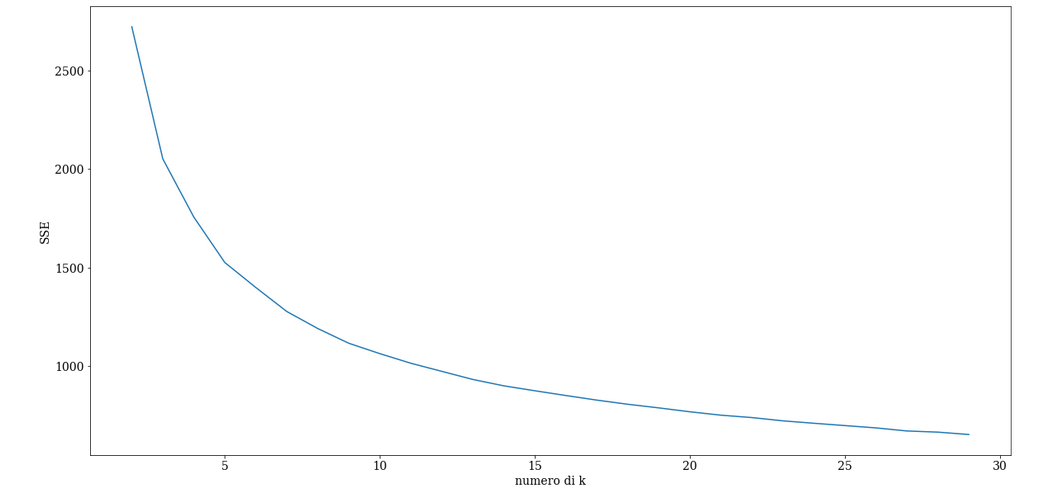
\includegraphics[width=14cm]{Images/Clustering/KMeansSSE.png}
		\vspace{-0.4cm}
		\caption{K-Means: SSE analisi.}
	\end{figure}\vspace{-0.6cm}$\newline$
	In base a questi risultati, il valore k di cluster da scegliere è 11, in quanto a partire da tale valore il SSE, che è più alto per un numero di clusters inferiore, si stabilizza intorno a 1000 e non subisce significative variazioni.$\newline$
	Per avere un ulteriore riscontro sul numero k di clusters da scegliere, oltre che con la misura del SSE, il risultato è stato messo in relazione alla misura della silhouette che permette di valutare il clustering sulla base non solo della coesione interna ad ogni cluster ma anche della separazione tra di essi. Essa assume in genere valori che vanno da -1 a 1 e, più è vicina a 1, migliore è il clustering.$\newline$
	L’algoritmo di k-means è stato dunque iterato per un numero di k che va da 5 a 15 e, per ogni iterazione, è stata memorizzata la silhouette, come mostra la seguente figura:\vspace{-0.2cm}	
	\begin{figure}[H]
		\centering
		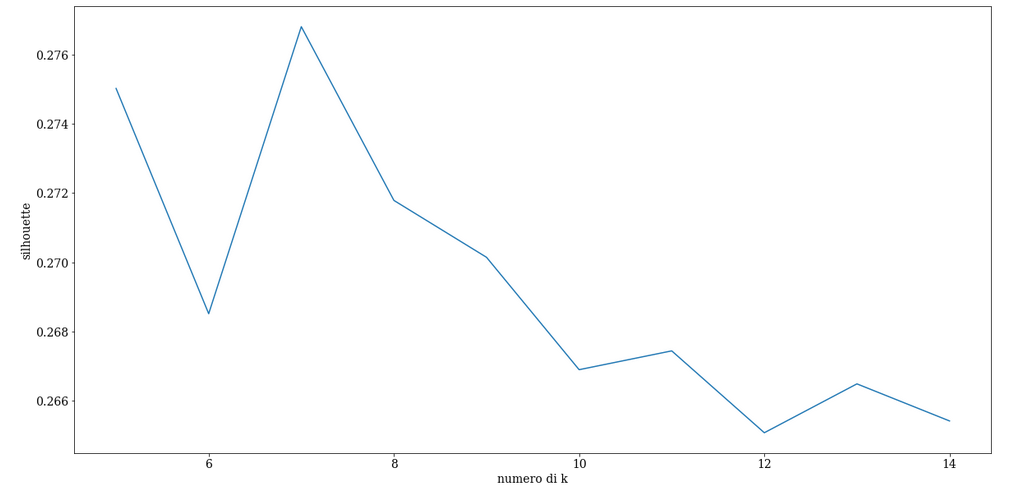
\includegraphics[width=14cm]{Images/Clustering/KMeansSilhouette.png}
		\vspace{-0.5cm}
		\caption{K-Means: Silhouette analisi.}
	\end{figure}\vspace{-0.6cm}$\newline$	
	Il valore della silhouette è in tutti i casi molto basso, infatti non supera lo 0.28. Tuttavia, si ha un picco per un numero di clusters pari a 7. Per 7 clusters, infatti, la silhouette ha un valore (arrotondato per eccesso) di 0.28, mentre per 11 clusters essa scende a 0.27. Per un numero di clusters pari a 7, però, come mostra la figura del SSE, si registra un aumento del SSE che si aggira intorno a 1200.$\newline$ 
	Premesso che si tratta di oscillazioni relativamente poco significative, è stato deciso di dare la priorità alla misura della silhouette per la scelta del numero k di clusters, in quanto essa fornisce una misura anche della separazione tra i clusters e in relazione a una silhouette di 0.28 il valore di SSE non subisce un aumento eccessivamente grande. Per questo motivo, è stato scelto di usare 7 clusters.
	
	
	\subsubsection{Caratterizzazione dei clusters ottenuti}
	Nella figura 6 sono mostrati i 7 clusters ottenuti applicando l’algoritmo k-means.
	\begin{figure}[H]
		\centering
		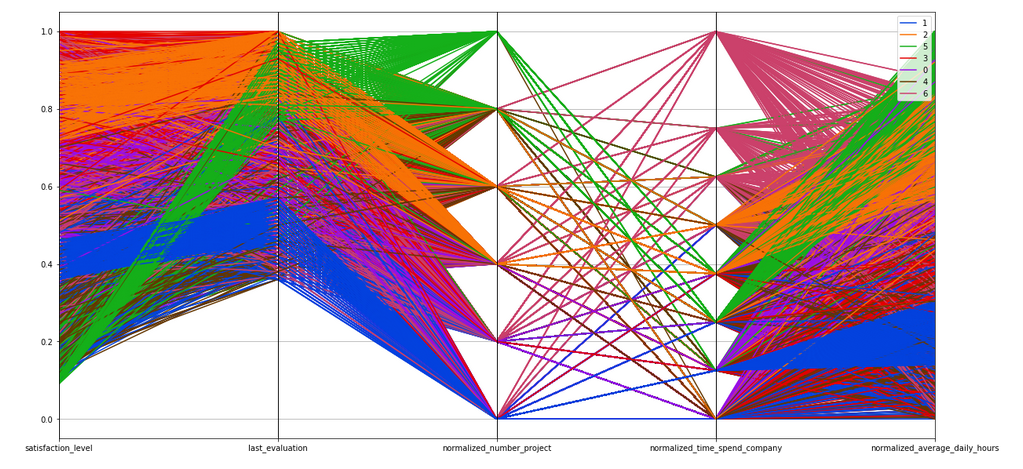
\includegraphics[width=14cm]{Images/Clustering/K-MeansParallel.png}
		\vspace{-0.5cm}
		\caption{Parallel coordinates dei cluster risultanti dal k-means.}
	\end{figure}\vspace{-0.5cm}$\newline$
	Come si può notare, il cluster 1, rappresentato dal colore blu, appare quello più nettamente distinto dagli altri, seguito dal 5, rappresentato dal verde, e dal 2, rappresentato dall’arancione. Per gli altri clusters invece, sono più evidenti sovrapposizioni ed essi appaiono, dunque, meno distinti gli uni dagli altri.\vspace{-0.2cm}
	\begin{itemize}
	\item Il cluster 0 contiene 3226 impiegati. La media di \textit{normalized\_average\_daily\_hours} è significativamente superiore a quella dell’intero dataset, essendo 11.13 contro 9.34. La maggior parte delle persone appartenenti a questo cluster non ha lasciato il lavoro (97.5\%).\vspace{-0.2cm}
	\item Il cluster 1 contiene 2562 impiegati. La media del numero di progetti è molto più bassa rispetto a quella calcolata sul dataset, infatti è 2.25 contro 3.8. Anche il numero di ore lavorative giornaliere è basso rispetto alla media totale del dataset, infatti è 6.95 contro 9.34. Più bassi sono anche i valori di \textit{satisfaction\_level} e \textit{last\_evaluation}, che sono rispettivamente 0.43 e 0.54 contro 0.61 e 0.72. Esso contiene inoltre, il maggior numero di impiegati, rispetto a tutti gli altri clusters, che hanno lasciato il lavoro (60.2\%).\vspace{-0.2cm}
	\item Il cluster 2 contiene 2323 impiegati. Le medie del numero di progetti e il numero di ore lavorative sono più alte rispetto a quelle calcolate sull’intero dataset, ovvero sono rispettivamente 4.7 e 11.23 contro 3.8 e 9.34. Anche le medie di \textit{satisfaction\_level} e \textit{last\_evaluation} superano significativamente quelle calcolate sull’intero dataset, essendo rispettivamente 0.80 e 0.85 contro 0.61 e 0.72. Questo cluster è formato per la maggior parte da impiegati che non hanno lasciato il lavoro (61.3\%).\vspace{-0.2cm}
	\item Al cluster 3 appartengono 3433 impiegati. La media di \textit{satisfaction\_level} è più alta di quella calcolata sull’intero numero di record, infatti è 0.80 contro 0.61. Per quanto riguarda il numero di ore lavorative giornaliere inoltre, la media è 7.65, al di sotto di quella dell’intero dataset, cioè 9.34. Rispetto agli altri clusters, questo è quello che contiene il maggior numero di impiegati che non hanno lasciato il lavoro (98.7\%), che non hanno avuto una promozione negli ultimi cinque anni (98\%), che non hanno avuto incidenti sul lavoro (83.4\%) e che hanno il salario più basso (47.1\%).\vspace{-0.2cm}
	\item Il cluster 4 contiene 1480 impiegati. Le medie di \textit{satisfaction\_level} e del numero di ore di lavoro giornaliere sono inferiori rispetto a quella dell’intero dataset, infatti sono rispettivamente 0.40 e 7.95 contro 0.61 e 9.34. La media del numero di progetti, invece, supera quella calcolata sull’intero dataset ed è 4.65 contro 3.8.  La maggior parte degli impiegati di questo cluster non ha lasciato il lavoro (94.7\%).\vspace{-0.2cm}
	\item Al cluster 5 appartengono 1283 impiegati. La media del livello di soddisfazione è molto più bassa rispetto a quella dell’intero dataset essendo 0.14 contro 0.61. Significativamente più alte sono invece, le medie del numero di progetti realizzati e del numero di ore giornaliere lavorative, che sono rispettivamente 5.95 e 12.53 contro 3.8 e 9.34. La maggior parte degli impiegati appartenenti a questo cluster ha lasciato il lavoro (71.9\%). Questo cluster, inoltre, contiene il minor numero di persone che hanno avuto promozioni negli ultimi cinque anni (solamente lo 0.9\%) e che hanno un salario alto (5.1\%).\vspace{-0.2cm}
	\item Il cluster 6 contiene 692 impiegati. Le medie di tutti gli attributi sono pressappoco allineate con quelle dell’intero dataset, eccetto per il numero di anni trascorsi presso la compagnia, per cui la media, che è 7.92, supera significativamente quella del dataset, ovvero 3.5. La maggior parte degli impiegati appartenenti a questo cluster ha un salario medio (51.3\%). Inoltre, a questo cluster appartengono il minor numero di impiegati (solo lo 0.9\%), rispetto a tutti gli altri clusters, che hanno lasciato il lavoro.
\end{itemize}\vspace{-0.2cm}
	Il cluster 1 e il cluster 5, che sono gli unici due in cui il maggior numero di impiegati ha lasciato il lavoro, possono essere usati per delineare due tipi principali di impiegati che lasciano il lavoro. Nel primo caso, si tratta di persone che hanno un livello di soddisfazione, una valutazione, un numero di progetti ed anche una quantità di ore lavorative giornaliere inferiori rispetto alla media. Nel secondo caso, quello delineato dal cluster 5, si tratta di impiegati che hanno un numero di progetti e di ore giornaliere lavorative superiori rispetto alla media, ma tra i quali si ha il minor numero di persone, rispetto a tutti gli altri impiegati, che ha avuto una promozione negli ultimi cinque anni e che percepisce un salario alto. Appare ovvio, dunque, come per questo cluster il livello di soddisfazione sia molto più basso rispetto alla media.$\newline$
	I cluster 2 e 3 invece, formati per la maggior parte da impiegati che non hanno lasciato il lavoro, mostrano chiaramente come questa scelta corrisponda a livelli di soddisfazione e valutazione più alti rispetto alla media.$\newline$
	Il cluster 6, infine, contenente il minor numero di impiegati, rispetto agli clusters, che hanno lasciato il lavoro, delinea un’altra caratteristica di questi impiegati, infatti la maggior parte di quelli appartenenti a questo cluster ha un salario alto e ovviamente, lavora da più anni nella compagnia rispetto ad altri.

\subsection{Clustering con DBscan}
	Il secondo algoritmo di clustering usato è il DBSCAN. Esso individua i cluster come regioni ad alta densità di punti, permettendo di separarli da aree a bassa densità che costituiscono il noise. L’algoritmo non richiede che sia fissato in precedenza il numero di cluster che si vogliono ottenere, ma è necessario fissare un raggio epsilon (\textit{eps}), e un numero minimo di punti \textit{minPts} che devono essere contenuti entro tale raggio. In base a questi valori i punti vengono suddivisi in core, border e noise.$\newline$
	%\subsubsection{Scelta degli attributi e della funzione di distanza}
	Il DBSCAN non è stato effettuato utilizzando l’intero dataset ma solamente su un gruppo ristretto di features: \textit{satisfaction\_level}, \textit{last\_evaluation}, \textit{normalized\_number\_project}, \textit{normalized\_time\_spent\_company} e \textit{normalized\_average\_daily\_hours}.$\newline$
	Sono stati quindi eliminati gli attributi categorici, quelli binari e l’attributo left in quanto target dell'analisi.$\newline$
	Le proprietà \textit{satisfaction\_level} e \textit{last\_evaluation}, come già descritto, hanno un range di valori che va da 0 a 1 e si è reso quindi necessario normalizzare \textit{number\_project}, \textit{time\_spent\_company} e \textit{average\_daily\_hours}.
		
	\subsubsection{Studio dei parametri}
	Per il calcolo ottimale dell'epsilon ci si è avvalsi dell’algoritmo k-nearest neighbor; sono state eseguite molteplici prove per valori di \textit{minPts} che vanno da 5 a 100 aumentando ad ogni prova successiva il valore di 5.$\newline$
	Ad ogni prova è stato individuato il miglior \textit{eps} analizzando la curva ricavata da k-nearest neighbor per quel valore di \textit{minPts} e ne è stato calcolato il DBSCAN e la corrispondente silhouette.$\newline$
	Infine sono stati scelti i valori di \textit{eps} e \textit{minPts} che hanno ottenuto il miglior punteggio di silhouette della serie. Nel nostro caso abbiamo ottenuto per \textit{eps} 0.2 e \textit{minPts} 75 con una silhouette di 0.243.
	\begin{figure}[H]
		\centering
		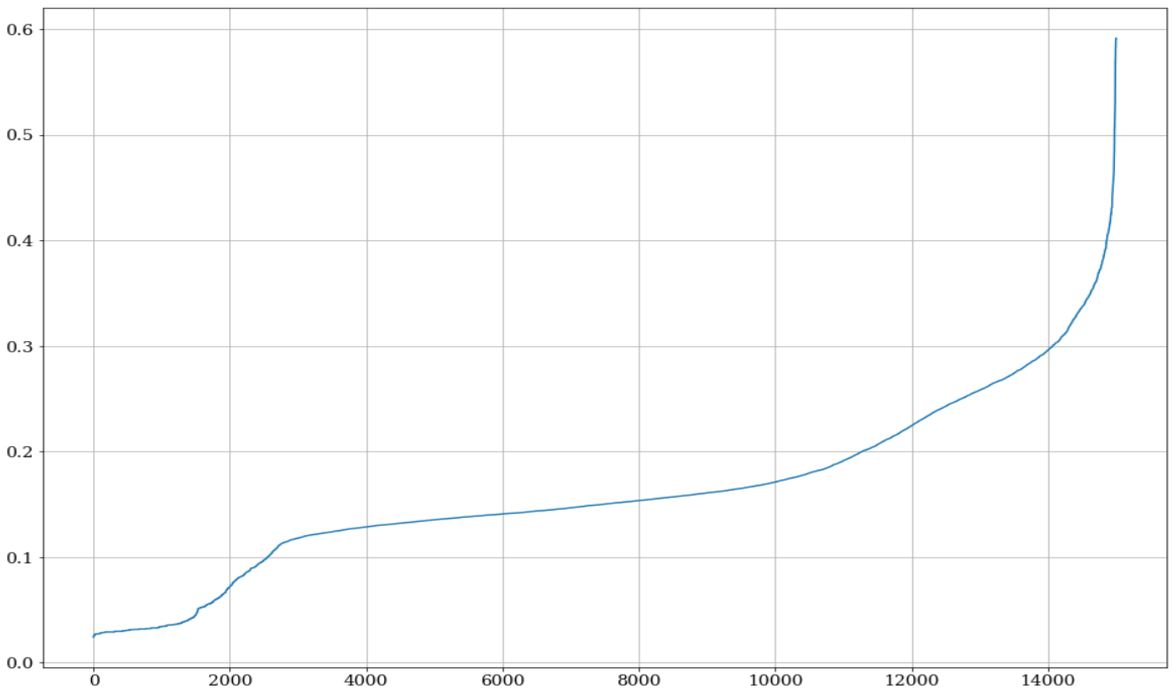
\includegraphics[width=12cm]{Images/Clustering/DBKnearest.jpg}
		\vspace{-0.3cm}
		\caption{DBSCAN. K-nearest neighbor con minPts: 75.}
	\end{figure}
	
	\subsubsection{Caratterizzazione dei clusters ottenuti}
	Questi valori hanno fornito una clusterizzazione del dataset in un cluster maggiore formato da 11545 record ed uno minore di 959 record oltre a 2495 nodi identificati come noise.$\newline$	
	Prendendo invece \textit{eps} pari a 0.19 il dataset viene suddiviso in 6 cluster (oltre al noise), che tuttavia risultano sparsi e frammentari, al contrario invece dei valori scelti in cui i 959 record ottenuti nel cluster minore hanno valori di features molto simili fra loro con uno scostamento di questi ultimi molto ridotto in confronto agli altri cluster.
	\begin{center}
		\begin{tabular}{cc}
			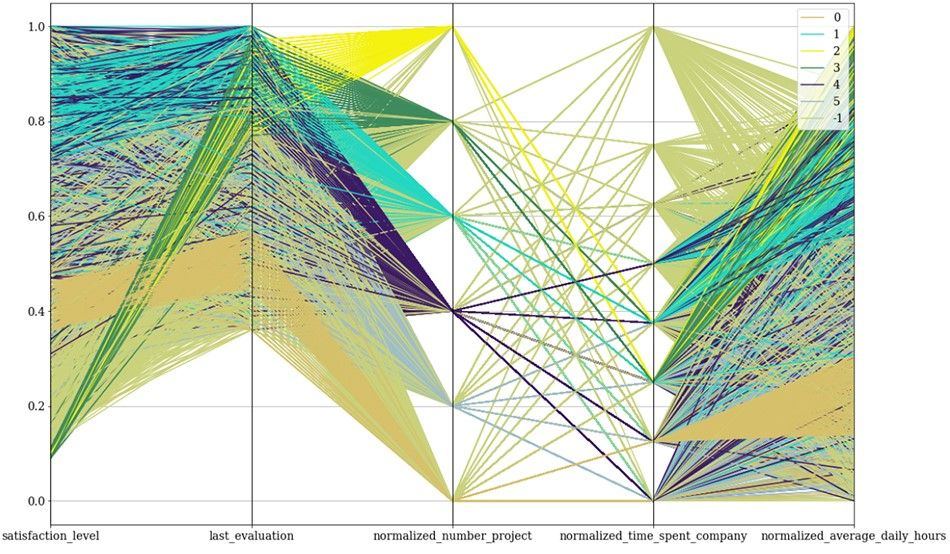
\includegraphics[width=0.5\linewidth]{Images/Clustering/DB_Parallel_Confronto_a.jpg} &
			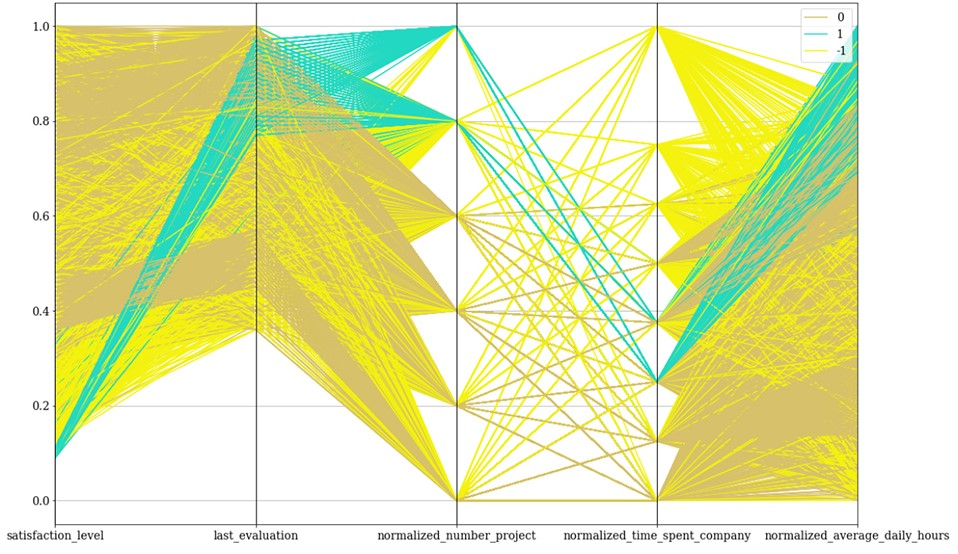
\includegraphics[width=0.5\linewidth]{Images/Clustering/DB_Parallel_Confronto_b.jpg} \\
			a) & b)\\
		\end{tabular}
		\vspace{-0.2cm}
		\captionof{figure}{DBSCAN. Confronto dei risultati: a sinistra (a) si è utilizzato un \textit{eps} di 0.19, a destra (b) un \textit{eps} di 0.2, in entrambi i casi \textit{minPts} è fissato a 75.}
	\end{center}$\newline$
	In figura 9 sono stati riportati i nodi del cluster in questione rapportati con l’attributo left, dove risulta che su un totale di 959 persone, 850 di questi hanno lasciato l’azienda e soltanto 109 hanno deciso di rimanere.$\newline$
	Come si nota dal grafico, coloro che hanno deciso di lasciare hanno valori fortemente simili tra loro per tutte le features prese in esame, ovvero \textit{satisfaction\_level} tendenzialmente basso, \textit{last\_evaluation} elevato, 6 e 7 progetti (i più alti del dataset), \textit{normalized\_time\_spent\_company} ristretto al range 0.25-0.37 e soltanto i valori più alti delle ore lavorative medie giornaliere.
	\begin{figure}[H]
		\centering
		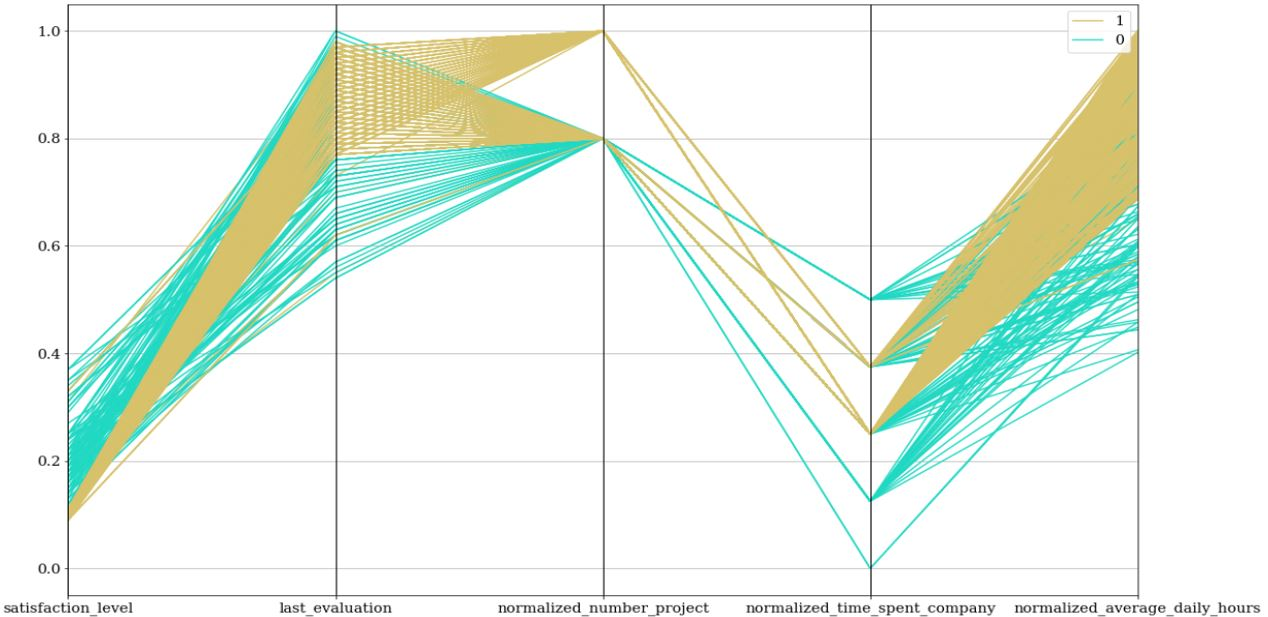
\includegraphics[width=15cm]{Images/Clustering/DBParallelLeft.jpg}
		\vspace{-0.2cm}
		\caption{DBSCAN. Dettaglio del cluster formato da 959 record, in celeste sono evidenziati i dipendenti che sono rimasti, in oro quelli che hanno deciso di lasciare.}
	\end{figure}
	
\subsection{Clustering con Hierarchical}
	Il terzo algoritmo di clustering applicato sui dati è lo hierarchical di tipo agglomerative. Esso considera inizialmente ogni punto come un singolo cluster e ad ogni iterazione riunisce i due clusters più vicini (cioè tra i quali vi è la minore distanza o la maggiore similarità), in modo da ottenere un insieme di clusters annidati organizzati in una struttura ad albero. A differenza di altri algoritmi di clustering, come il k-means, esso non richiede di specificare a priori il numero di clusters che si vogliono ottenere.$\newline$ 
	%\subsubsection{Choice of attributes and distance function}
	Le variabili scelte per eseguire questa analisi sono quelle numeriche non binarie. I valori binari infatti sono per natura suddivisi in 2 cluster, mentre per quelli categorici non è possibile stabilire un criterio per calcolare la distanza. $\newline$ 
	Gli attributi numerici sono stati normalizzati poiché valori appartenenti a scale diverse potrebbero sbilanciare la matrice delle distanze verso un particolare attributo. I valori quindi utilizzati sono: \textit{satisfaction\_level}, \textit{last\_evaluation}, \textit{normalized\_average\_daily\_hours}, \textit{normalized\_number\_project}, \textit{normalized\_time\_spent\_company}. $\newline$
	Per scegliere quale funzione utilizzare per calcolare la matrice delle distanze si sono svolti esperimenti con la distanza euclidea, la manhattan e la cosine. Per testare quale fosse la più adatta si è eseguita un'analisi della silhouette. Da questa si è compreso che con la cosine si ottengono i valori più bassi anche per un numero minore di cluster. La manhattan e la euclidea invece sono paragonabili, i risultati variano leggermente a seconda del criterio di collegamento utilizzato. $\newline$
	Alla fine si è scelto di utilizzare la distanza euclidea poiché è il metodo di misurazione più standard e ci permette di testare anche il criterio di Ward per calcolare i cluster.
	
	
	\subsubsection{Scelta tra i diversi algoritmi}
	Per testare quale funzione di collegamento utilizzare anche in questo caso abbiamo eseguito diversi esperimenti e osservato i cluster che si formavano al variare dell'algoritmo e del numero di cluster scelto. $\newline$
	Il complete linkage restituisce per qualunque numero di cluster dei valori della silhouette vicini allo zero, il che indica che molti record erano associati a cluster sbagliati. L'average linkage d'altra parte crea cluster poco uniformi. Già con valori bassi di $n\_cluster$ si formano cluster di dimensione irrisoria. Il single linkage infine presenta entrambe le problematiche.$\newline$
	Queste analisi sono confermate anche dai relativi dendrogrammi, infatti nel complete si nota che la divisione tra i cluster non è ben definita, nell'average è presente un cluster molto ampio e alcuni di dimensione talmente ridotta che non sono neanche visibili nel grafico e nel single vi sono tantissimi cluster minuscoli e le distanze tra cluster diversi sono molto ridotte.
	\begin{figure}[H]
		\centering
		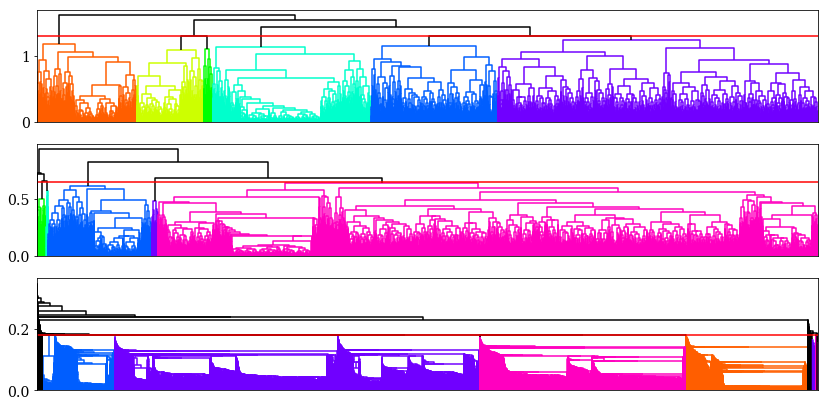
\includegraphics[width=16cm]{Images/Clustering/Hiercarchical_AvgComp.png}
		\vspace{-0.7cm}
		\caption{Dendrogramma con distanza euclidea e criterio di linkaggio Complete (a), Average (b) e Single (c). \`{E} stata fissata una soglia di threshold solo per rendere più chiara la lettura dei grafici.}
	\end{figure}\vspace{-0.5cm}$\newline$
	Infine si è sperimentato l’algoritmo con il criterio di Ward. Questo metodo, per scegliere quali coppie di cluster unire ad ogni passo, si basa sul valore ottimale di una funzione obiettiva. Le funzioni utilizzate possono essere diverse, quella più standard è la somma al quadrato degli errori, infatti il criterio di Ward è anche chiamato metodo della minima varianza. $\newline$
	Questo metodo ha restituito i risultati migliori. Infatti, anche verificando visivamente tramite dedrogramma, si può notare che in questo caso le distanze tra cluster diversi sono maggiori rispetto agli altri metodi, mentre sono minimizzate quelle interne. Inoltre le dimensioni dei vari cluster sono piuttosto omogenee.
	\begin{figure}[H]
		\centering
		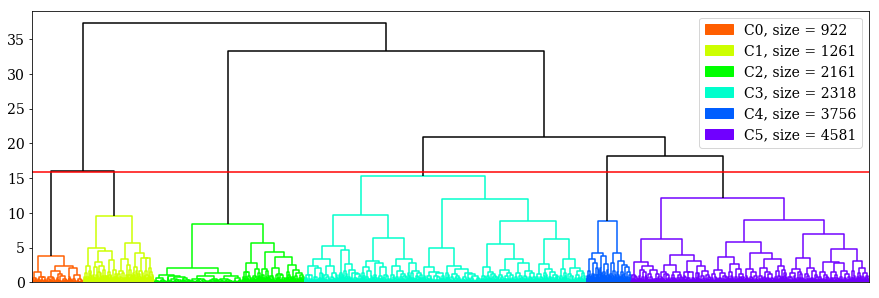
\includegraphics[width=17cm]{Images/Clustering/Hiercarchical_Ward.png}
		\vspace{-0.5cm}
		\caption{Dendrogramma con distanza euclidea e criterio di Ward.}
	\end{figure}\vspace{-0.5cm}$\newline$
	Per scegliere quale sia il numero di cluster ideale si possono sfruttare diversi criteri. $\newline$
	Innanzi tutto si è osservato il dendrogramma e si è cercato di dividere i cluster aventi maggiore distanza. Questo ci ha portato a suddividere il nostro database dai 3 ai 7 cluster. Come ulteriore conferma di questa ipotesi abbiamo sfruttato le analisi sulla silhouette fatte in precedenza. Siccome per $ n\_cluster = 5, 6, 7, 11, 14 $ o $ 15 $ la silhouette presenta un jump positivo, il che implica che tali valori sono buoni candidati, restringiamo la nostra scelta tra 5, 6 o 7.$\newline$
	Infine abbiamo deciso che il numero ottimale di cluster sarebbe stato 6 osservando la distribuzione dei cluster in una scatter matrix. 
	
	
\subsection{Valutazione finale del miglior metodo di clustering}
	Mettendo i vari metodi di clustering a confronto si può notare come tutti e tre hanno raggruppato i record in un numero che va dai 6 ai 7 cluster.
	Analizzando i risultati più nello specifico, tuttavia, si nota che:
	\begin{itemize}
		\item Il K-means ci ha fornito 7 cluster, tra i quali 2 risultano avere un consistente numero di persone che hanno lasciato. Il primo denota una tipologia di persone con livelli di soddisfazione, valutazione, numero di progetti e ore giornaliere lavorative inferiore alla media. L’altro gruppo, al contrario, raggruppa persone con numero di progetti e ore giornaliere lavorative tra le più alte del dataset.
		\item Nel caso del DBSCAN, i 6 cluster creati (più i noise) risultano frammentari e sparsi senza nette distinzioni. Questo ci ha portato ad optare (come confermato dal k-nearest neighbor) per un \textit{eps} maggiore ed un risultato di due soli cluster che hanno messo in evidenza un raggruppamento (seppur ristretto) molto omogeneo di persone che hanno abbandonato l’azienda. Questo raggruppamento somiglia, per caratteristiche, ad uno di quelli ricavati dal K-means.
		\item L’algoritmo di Hierarchical Clustering, con l’ausilio del criterio di Ward, è quello che ha dato i risultati migliori. Questo metodo ci ha fornito 6 cluster dove le distanze interne sono minimizzate fornendo raggruppamenti più equilibrati, mentre sono accentuate quelle fra cluster diversi. Dal dendrogramma si può notare anche come questi ultimi risultino avere dimensioni più omogenee rispetto agli altri risultati.
	\end{itemize}
	
	

	